\documentclass[conference,10pt]{IEEEtran}
\usepackage{amsmath,amssymb,graphicx,booktabs}
\usepackage{newtxtext,newtxmath}
\usepackage[hidelinks]{hyperref}
\usepackage[font=footnotesize]{caption}
\setlength{\textfloatsep}{6pt}
\makeatletter\def\@IEEEsectpunct{}\makeatother
\usepackage{titlesec}\titlespacing*{\section}{0pt}{4pt}{2pt}
\setlength{\abovedisplayskip}{3pt}\setlength{\belowdisplayskip}{3pt}

\begin{document}
\title{\vspace{-0.45in}\LARGE Litmus: KV-Cache Reuse and the Accuracy-Latency\\Frontier of On-Device Manipulation Detection}
\author{\IEEEauthorblockN{Devansh Gaur}
\IEEEauthorblockA{University of Waterloo, Waterloo, ON, Canada\vspace{-6pt}}}
\twocolumn[{\renewcommand\twocolumn[1][]{#1}\maketitle\vspace{-16pt}
\begin{center}
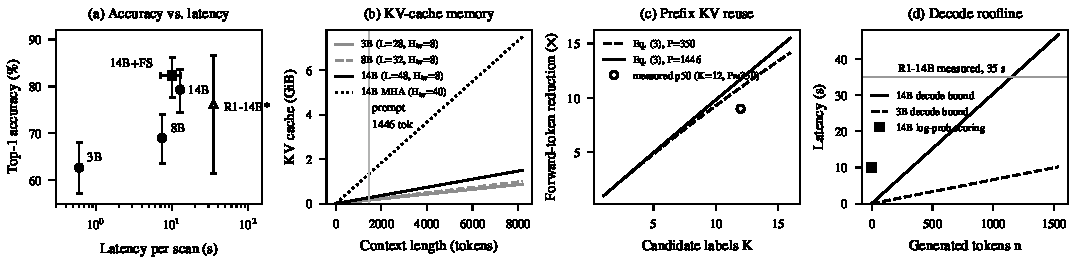
\includegraphics[width=\textwidth]{fig_main.pdf}
\vspace{-6pt}
\captionof{figure}{(a) Accuracy vs.\ latency on Apple M4 Pro, Wilson 95\% intervals (*R1: balanced $N{=}42$ subset). (b) fp16 KV cache from each \texttt{config.json}; dotted is a 14B multi-head counterfactual. (c) Eq.~(3) vs.\ measured p50 speedup. (d) Eq.~(4) decode bound.}\label{fig:main}
\end{center}\vspace{-4pt}}]

\noindent\textbf{\textit{Abstract:}} \textbf{Litmus labels a text selection with one of 14 persuasion techniques or \emph{none} by scoring candidate labels under a local 4-bit LLM. This note analyzes KV-cache memory, prefix KV reuse, and the decode bandwidth bound. Held-out top-1 accuracy rose from 62.7\% (3B) to 82.3\% (14B, few-shot); prefix reuse cut median latency 9.0$\times$.}

\section{Scoring as Constrained Decoding}
The detector never generates text. For input $x$ and each label $y\in\mathcal{Y}$ ($K{=}|\mathcal{Y}|{=}15$) it computes
\begin{equation}
s(y\mid x)=\tfrac{1}{|y|}\textstyle\sum_{t=1}^{|y|}\log p_\theta(y_t\mid x,y_{<t})
\end{equation}
and returns $\arg\max_y s$. Length normalization removes the bias toward short labels (1 to 7 tokens). A two-label gate first screens benign text (PR-AUC 0.93). Ranked scores give top-2 accuracy of 73.0\% against 64.0\% top-1 on the 3B, so most errors name a co-present technique.

\section{KV-Cache Memory}
Each attention layer caches one key and one value per token:
\begin{equation}
M_{\mathrm{tok}}=2\,L\,H_{kv}\,d_h\,b .
\end{equation}
All three models use grouped-query attention \cite{gqa} with $H_{kv}{=}8$, $d_h{=}128$, giving 112, 128 and 192\,KiB per token (3B, 8B, 14B, fp16). The 1446-token few-shot prompt occupies 271\,MiB on the 14B, against 1.32\,GiB under full multi-head attention with $H_{kv}{=}40$ (Fig.~\ref{fig:main}b). Beside 8.31\,GB of weights the cache is minor, so RAM did not limit the 14B on a 24\,GB machine.

\section{Prefix KV Reuse}
All labels share a $P$-token prefix. The deployed scorer prefills it once, appends each label to the cache, reads its log-probabilities, then trims the cache back to length $P$. Verdicts are unchanged. Relative to $K$ independent passes, forwarded tokens fall by
\begin{equation}
S(K)=\frac{K(P+\bar\ell)}{P+K(\bar\ell-1)} .
\end{equation}
At $P{=}1446$ the scorer forwards 1493 tokens instead of 21{,}752 (14.6$\times$). At measurement time ($K{=}12$, $P{\approx}350$) Eq.~(3) predicted 11.0$\times$; median latency fell from 4014 to 446\,ms (9.0$\times$, Fig.~\ref{fig:main}c). The gap is fixed per-call overhead and label tokens attending over the full prefix.

\section{Prefill Versus Decode}
Prefill is parallel and compute-bound. Decode emits one token per step and streams all weights each step:
\begin{equation}
t_{\mathrm{dec}}(n)\ \ge\ nW/B .
\end{equation}
With $W{=}8.31$\,GB and $B{=}273$\,GB/s, the 14B needs at least 30.4\,ms per token. Log-prob scoring decodes zero tokens. DeepSeek-R1-Distill-14B \cite{r1} must decode a chain of thought first: it averaged 35\,s per scan, which bounds its mean chain at about 1150 tokens (Fig.~\ref{fig:main}d), and reached only 76.2\% on a balanced subset.

\begin{table}[!b]
\centering\footnotesize
\caption{Held-out benchmark ($N{=}300$), all on-device}
\label{tab:res}
\vspace{-4pt}
\begin{tabular}{@{}lccc@{}}
\toprule
Configuration & Top-1 (\%) & MCC & Latency (s)\\
\midrule
3B, few-shot (shipped) & 62.7 & 0.55 & 0.6\\
\quad + gate fix, clean set & 66.9 & n/a & 0.6\\
8B, zero-shot & 69.0 & 0.634 & 7.4\\
14B, zero-shot & 79.3 & 0.752 & 12.7\\
\textbf{14B, few-shot} & \textbf{82.3} & \textbf{0.787} & 7 to 13\\
14B, LoRA ($N{=}123$) & 78.9 & n/a & n/a\\
\bottomrule
\end{tabular}
\end{table}

\section{Results and Discussion}
Accuracy rose monotonically with size (Table~\ref{tab:res}), so 62.7\% was a 3B capacity limit. Few-shot exemplars helped the 14B by three points but not the 3B. LoRA \cite{lora} on 503 imbalanced examples did not beat few-shot, and self-consistency voting \cite{sc} gained nothing on cleaned labels. The 3B serves the 0.6\,s shortcut and the 14B is an opt-in deep scan: the split is set by compute and bandwidth, not memory.

\vspace{-2pt}
\begin{thebibliography}{9}
\scriptsize
\setlength{\itemsep}{0pt}
\bibitem{gqa} J.~Ainslie \emph{et al.}, ``GQA: Training generalized multi-query transformer models from multi-head checkpoints,'' in \emph{Proc. EMNLP}, 2023.
\bibitem{r1} DeepSeek-AI, ``DeepSeek-R1: Incentivizing reasoning capability in LLMs via reinforcement learning,'' arXiv:2501.12948, 2025.
\bibitem{lora} E.~J.~Hu \emph{et al.}, ``LoRA: Low-rank adaptation of large language models,'' in \emph{Proc. ICLR}, 2022.
\bibitem{sc} X.~Wang \emph{et al.}, ``Self-consistency improves chain of thought reasoning in language models,'' in \emph{Proc. ICLR}, 2023.
\end{thebibliography}
\end{document}
